\chapter{Prototype Development}


boilerplate text, boilerplate text, boilerplate text, boilerplate text, boilerplate text, boilerplate text, boilerplate text, boilerplate text, boilerplate text, boilerplate text.


\section {Prototype Requirements}

\subsection{Risk Analysis}

Mention other risk analysis tools \cite{l2beatL2BEATStateLayer2024}

TODO:
* Asset storage (private servers, IPFS, Arweave)
* Libraries/Dependencies
* Networked Dependencies (type, blockchain indexer vs other APIs, public endpoints or private)
* Open source or not (obfuscated code, code running on private infra)




\section {Prototype 1 - genartdex}

\section{System Architecture}

boilerplate text, boilerplate text, boilerplate text, boilerplate text, boilerplate text, boilerplate text, boilerplate text, boilerplate text, boilerplate text, boilerplate text.


\subsection{Webpage metadata}

A common issue with most web pages, which can cause considerable annoyance to researchers who are working under tight deadlines, is the fact that they often lack the required metadata that is used by reference management tools, like Zotero, to automatically pull the metadata and populate the bibliographical record.

By default Arkivo suffered from the same problem, so attention was given to resolving this.
The \texttt{ArtifactController} now prepares a special data structure, \texttt{citationMetadata}, with all the required data fields, which is then used by the \texttt{header} section of the Edge template.
After experimenting with different metadata standards \cite{DevExposing_metadataZotero}\cite{zahidOpenGraphMeta2023} , a solution was found using a mixture of standards, where Zotero can pull most of the relevant fields related to an artifact, as shown in \autoref{fig:zotero-metadata-comparison}


\begin{lstlisting}[style=htmlCode,caption={Artifact page metadata}] 
<title>{{ citationMetadata.title}} - arkivo.art</title>
<meta property="og:title" content="{{ citationMetadata.title }}">
<meta property="og:type" content="website">
<meta property="dc.creator" content="{{ citationMetadata.author }}">
<meta property="article:published_time" content="{{ citationMetadata.date }}">
<meta property="og:description" content="{{ citationMetadata.description }}">
<meta property="og:site_name" content="arkivo.art">
\end{lstlisting}


\begin{figure}[H]
  \centering
  \begin{subfigure}[b]{0.45\textwidth}
    \centering
    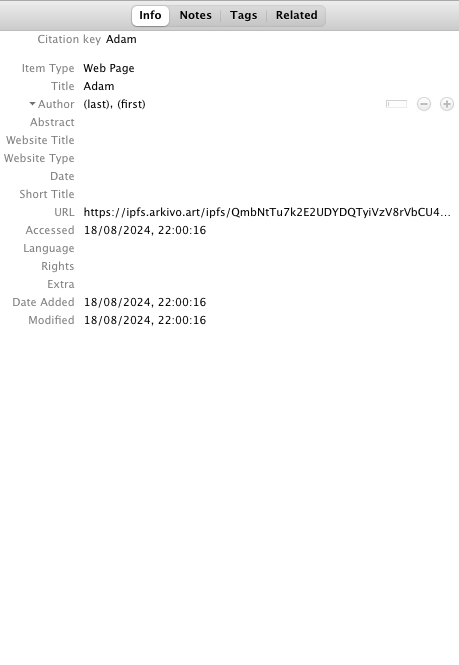
\includegraphics[width=\textwidth]{page-metadata-before.png}
    \caption{Before header metadata}
    \label{fig:image1}
  \end{subfigure}
  \hfill
  \begin{subfigure}[b]{0.45\textwidth}
    \centering
    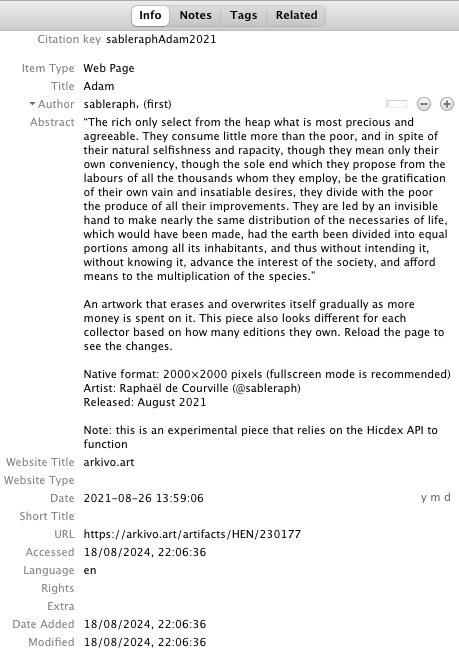
\includegraphics[width=\textwidth]{page-metadata-after.png}
    \caption{After header metadata}
    \label{fig:image2}
  \end{subfigure}
  \caption{Artifact metadata pulled by Zotero}
  \label{fig:zotero-metadata-comparison}
\end{figure}



\subsection{Encapsulation of internal IDs}

In normal circumstances the listing of a model, like Artifact, would include the unique ID of that model as stored in the database, for example: \texttt{/artifacts/45}

However this ID is unique to this instance of the application, and it can vary based on the timing of artifact discovery between other instances.
For this reason it is imperative that none of the internal IDs generated by the database are exposed to the user.

In order to achieve this, all URLs must be generated using only public identifiers which uniquely identify a model, in the case of an artifact: \texttt{blockchain /  smart contract / tokenId}.
This scheme closely follows existing proposals for cross-chain standardisation of identifiers \cite{herzogAssetTypeAsset2020}.

So what would be a URL:

\texttt{/artifacts/2065}

Becomes:

\texttt{/artifacts/tezos/KT1RJ6PbjHpwc3M5rw5s2Nbmefwbuwbdxton/230177}


However this URL is quite verbose. For convenience, since most of our initial artifacts are all on tezos, and on the HEN's OBJKT smart contract we can:

\begin{itemize}
    \item omit the blockchain identifier
    \item use an alias for the smart contract address
\end{itemize}

This strategy allows us to have shorter, but still unique URLs, which do not expose our internal DB IDs.

\texttt{/artifacts/HEN/230177}

Of course, the long-form URL should also work.

\subsection{Infrastructure}

A typical centralised application would be sensible to settle for state-of-the-art deployment platforms like Amazon ACS, DigitalOcean, Heroku, or Microsoft Azure. Not only do these commercial infrastructure solutions offer reliable up-time with fast Internet access, but also a wide range of geographically dispersed data centres across the world for maximum resiliency. It is theoretically possible to deploy a distributed and decentralised (control) solution across these platforms from an application point of view, however at the infrastructure level, the control would be centralised on a small number of industry players, which are an easy target for censorship requests from governments (ref needed).

\subsection{Smart Contracts}

boilerplate text, boilerplate text, boilerplate text, boilerplate text, boilerplate text, boilerplate text, boilerplate text, boilerplate text, boilerplate text, boilerplate text.

\subsection{Authentication}

todo: authentication vs authorisation vs access control

One of the main benefits of web3-style authentication is that it does not require any user credentials stored in the application's database. Since all web3 users have their public keys publicly registered on the blockchain, any user can identify themselves by \emph{connecting} their web3 wallet and signing a custom message provided by the application. This way the application can verify who the user is and that they are in possession of the private key, therefore validating their authentication credentials.

\section{Open Source}

Open sourcing this project was essencial because...

\subsection{Open Source License}

The choice of license...


The choice of license for this project was ... due to...



\section{Security: Detecting and Dealing with Malicious Code}

In this section I will talk about the security aspects of code-base artworks.